\section{Results}\label{sec:results}

This section reports the welfare and fiscal effects of the five instrument eliminations and of the 66 reforms, from the value of the existing instruments to a map of all reforms. Every entry in the tables and figures below comes from simulating the estimated model of Sections~\ref{sec:model} and~\ref{sec:estimation} for the cohort under the reform, announced before age 30 and in force over the whole life cycle, with wages and the interest rate held fixed. The reform tables share one format. WTP is the ex ante consumption-equivalent welfare change at age 30, in percent of consumption at every age (Section~\ref{sec:fw_welfare}). The three fiscal columns are percentage changes in present values at age 62: Direct refers to the program that the reform changes, including the behavioral responses within that program; Indirect to all other taxes and transfers; and Net to total government spending (Section~\ref{sec:fw_fiscal}). The MVPF converts WTP into dollars with the present value of baseline per capita consumption and divides it by the dollar change in government spending (equation~\eqref{eq:mvpf}). It is infinite when WTP is positive and the net cost negative; for a reform that lowers welfare and saves money, it is the welfare cost per dollar saved. The last three columns report changes in labor force participation, in percentage points, at ages 30--49, 62--64, and 65--69.

% ---------------------------------------------------------------------------
\subsection{The Value of Existing Instruments}\label{sec:results_elim}

We first measure what each existing instrument contributes to welfare by removing it, one at a time, from the estimated economy. \autoref{tab:elim} reports the results. Eliminating Social Security benefits (D1) lowers welfare by 5.89 percent of consumption, the largest change among the five experiments. Eliminating only the retirement benefits, and keeping disability benefits, lowers welfare by 5.34 percent in consumption-equivalent and 6.15 percent in leisure-equivalent terms. % Source: FROT 2025_sub/7_policy_reforms.tex (footnote in Welfare Decomposition)
Social Security benefits are an annuity whose level depends on lifetime earnings through a progressive formula. They insure longevity risk, which individuals can otherwise self-insure only by holding wealth that is lost at death, and they insure part of the consequences of low ability and poor health for lifetime earnings.

\begin{table}[!htbp]
\centering
\caption{Welfare Value of Existing Policy Instruments}\label{tab:elim}
\small
% Source: FROT tables/welfare_decomposition_gradient.tex (May 2025 simulation of the estimated model). Authors: rerun on corrected code before submission if results changed.
% Source: FROT tables/welfare_decomposition_gradient.tex.
% AUTHORS: reform and elimination results are from the May 2025 simulation; fit figures are the 2026 corrected re-simulation. Rerun reforms on the corrected code before submission.
% Values copied exactly from the source (CE and LE columns); D2 keeps the source sign convention (loss from incomplete coverage).
\begin{tabular}{@{}l l c c@{}}
\toprule
 & Experiment & CE (\%) & LE (\%) \\
\midrule
(D1) & No Social Security benefits & $-$5.89 & $-$6.79 \\
(D2) & Incomplete Medicare coverage after 65 (loss relative to full coverage) & $-$4.28 & $-$4.93 \\
(D3) & Full savings subsidy ($r=r_f$) & 3.60 & 4.15 \\
(D4) & No income tax & 3.16 & 3.64 \\
(D5) & No disability benefits & $-$0.34 & $-$0.40 \\
\bottomrule
\end{tabular}

\tabnotes{\textit{Notes:} Welfare change, in percent, from eliminating one policy instrument from the estimated economy, all other rules unchanged. CE is the ex ante consumption-equivalent change at age 30: the proportional change in consumption at every age that gives the same expected lifetime utility (equation~\eqref{eq:ce}). LE is the analogous leisure-equivalent change; because utility is homothetic, $\text{LE}=\text{CE}\times\gamma/(1-\gamma)$. D1 sets Social Security benefits to zero. D2 compares the status quo with an economy in which all medical expenditures after age 65 are covered for participants and nonparticipants; it is reported as the welfare loss from the incomplete coverage of the status quo, so full coverage would raise welfare by 4.28 percent (CE). D3 sets the net return on assets $r$ equal to the pretax return $r_f$. D4 sets the income tax to zero. D5 sets disability insurance benefits to zero. The experiments are not budget balanced. Each entry comes from simulating the estimated model for the cohort under the counterfactual, with prices held fixed. Participation profiles under each experiment are in \autoref{fig:elim_lfpr} and \autoref{fig:elim_lfpr_health}.}
\end{table}

Medicare ranks second. Covering all medical expenditures after age 65, for participants and nonparticipants alike, would raise welfare by 4.28 percent; \autoref{tab:elim} reports this gain with a negative sign, as the welfare loss from the incomplete coverage of the status quo. Out-of-pocket medical expenses rise steeply with age and are concentrated among individuals in poor health or with a disability (Section~\ref{sec:model_medical}), so their uninsured part is a large old-age risk \citep{Denardi2010}. A full subsidy to saving that raises the net return to the pretax return (D3) raises welfare by 3.60 percent, and abolishing the income tax (D4) raises it by 3.16 percent. Eliminating disability insurance (D5) lowers welfare by only 0.34 percent. The loss falls on individuals with a disability after age 50, a small share of the cohort, and the ex ante measure weights it by the probability of reaching that state. The leisure-equivalent changes are proportional to the consumption-equivalent ones and preserve the ordering.

The elimination of Social Security also moves participation the most (\autoref{fig:elim_lfpr} and \autoref{fig:elim_lfpr_health} in Appendix~\ref{app:figures}). Without benefits, participation falls slightly before age 50, when work no longer builds future benefits, and rises sharply from the 50s on, in every health state, as individuals must finance old-age consumption from their own earnings and savings. Eliminating DI raises the participation of individuals with a disability after age 50 substantially, which reflects its role as the main pathway out of the labor force for this group. The three experiments that raise welfare---full Medicare coverage, the full savings subsidy, and the abolition of the income tax---lower aggregate participation at older ages: each raises the resources available in old age, and the income effect dominates.

These rankings qualify the emphasis that \citet{french2011effects} place on Medicare in retirement decisions.\footnote{The working-paper version of their analysis, \citet{French2004}, finds a larger effect of Social Security than of Medicare on labor supply; the published version places more weight on Medicare, whose effect it finds to be close to that of Social Security.} Medicare matters in our economy: full coverage after 65 would be worth 4.28 percent of consumption. Social Security is nonetheless the more valuable instrument, and its elimination moves participation the most.

None of these experiments holds the government budget fixed. D3 and D4 transfer resources to households without financing them, and the other experiments change government spending without any offsetting change elsewhere in the budget. Their welfare effects measure the value of the instruments as they stand, not the desirability of changing them: the gain from D4 does not imply that the income tax should be abolished, because the experiment does not ask who pays for its abolition. The MVPF puts the welfare effect of each reform against its net cost to the government, and we use it for the rest of the section.

% ---------------------------------------------------------------------------
\subsection{Rewarding versus Mandating Delay}\label{sec:results_claiming}

The reforms of the claiming-age schedule produce the central result of the paper. \autoref{fig:schedules} shows how each family changes the benefit, in percent of the PIA, that an individual receives for each claiming age between 62 and 70. Raising the NRA (Panel A) shifts the whole schedule to the right, so that the benefit falls at every claiming age: under an NRA of 66 (AN1), a claim at 66 pays what a claim at 65 pays in the status quo. The DRC reforms AD1--AD5 (Panel B) raise the benefit at every claiming age above the NRA and leave it unchanged at and below the NRA. The symmetric reforms AL1--AL9 set the reduction for early claiming and the credit for delay to a common rate and rotate the schedule around the NRA, which stays at 65: under AL9, benefits range from 55 percent of the PIA at 62 to 175 percent at 70, against 80 and 122.5 percent in the status quo. At unchanged claiming ages, an NRA increase lowers the benefit of every claimant, whereas an AD reform raises the benefit of every claimant who claims after 65 and lowers no one's. An NRA increase mandates later retirement; a higher credit rewards it.

\begin{figure}[!htbp]
\centering
\caption{Claiming-Age Schedules under the Status Quo and Selected Reforms}\label{fig:schedules}
\vspace{0.5em}
% Generated from FROT tables/DRC_visualization_4.tex (program rules; see figures/schedules_A.tex and schedules_B.tex).
\begin{tabular}{@{}c@{\hspace{0.5em}}c@{}}
% Generated by gen_figs.py from FROT tables/DRC_visualization_4.tex (program rules: benefit as % of PIA by claiming age).
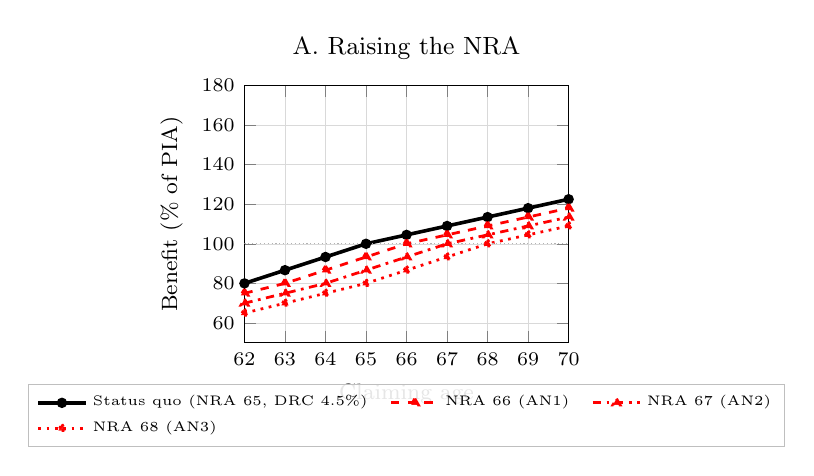
\begin{tikzpicture}
\begin{axis}[width=0.47\textwidth,height=0.40\textwidth,xmin=62,xmax=70,ymin=50,ymax=180,
  xtick={62,...,70},ytick={60,80,100,120,140,160,180},
  title={A. Raising the NRA},title style={font=\small},
  xlabel={Claiming age},ylabel={Benefit (\% of PIA)},
  grid=both,grid style={line width=.1pt, draw=gray!15},major grid style={line width=.2pt,draw=gray!30},
  tick label style={font=\scriptsize},label style={font=\footnotesize},
  legend style={font=\tiny,at={(0.02,0.98)},anchor=north west,draw=gray!50,fill=white,fill opacity=0.9,text opacity=1},legend cell align=left]
\addplot[black,line width=1.3pt,mark=*,mark size=1.2pt] coordinates {(62,80) (63,86.67) (64,93.33) (65,100) (66,104.5) (67,109) (68,113.5) (69,118) (70,122.5)};
\addlegendentry{Status quo (NRA 65, DRC 4.5\%)}
\addplot[red,line width=1pt,dashed,mark=triangle*,mark size=1.5pt] coordinates {(62,75) (63,80) (64,86.67) (65,93.33) (66,100) (67,104.5) (68,109) (69,113.5) (70,118)};
\addlegendentry{NRA 66 (AN1)}
\addplot[red,line width=1pt,dashdotted,mark=triangle*,mark size=1.5pt] coordinates {(62,70) (63,75) (64,80) (65,86.67) (66,93.33) (67,100) (68,104.5) (69,109) (70,113.5)};
\addlegendentry{NRA 67 (AN2)}
\addplot[red,line width=1pt,dotted,mark=triangle*,mark size=1.5pt] coordinates {(62,65) (63,70) (64,75) (65,80) (66,86.67) (67,93.33) (68,100) (69,104.5) (70,109)};
\addlegendentry{NRA 68 (AN3)}
\draw[gray!60,densely dotted] (axis cs:62,100) -- (axis cs:70,100);
\end{axis}
\end{tikzpicture}
 & % Generated by gen_figs.py from FROT tables/DRC_visualization_4.tex (program rules: benefit as % of PIA by claiming age).
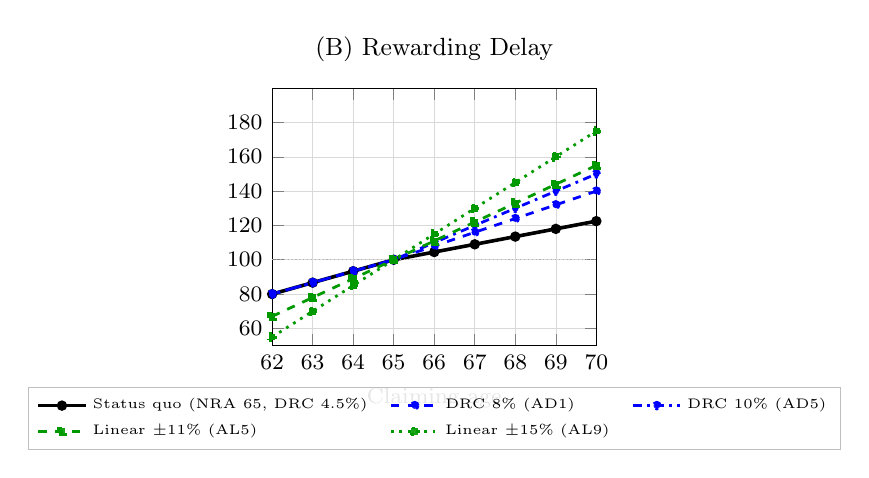
\begin{tikzpicture}
\begin{axis}[width=0.47\textwidth,height=0.40\textwidth,xmin=62,xmax=70,ymin=50,ymax=200,
  xtick={62,...,70},ytick={60,80,100,120,140,160,180},
  title={(B) Rewarding Delay},title style={font=\small},
  xlabel={Claiming age},
  grid=both,grid style={line width=.1pt, draw=gray!15},major grid style={line width=.2pt,draw=gray!30},
  tick label style={font=\footnotesize},label style={font=\footnotesize},
  legend style={font=\tiny,at={(0.02,0.98)},anchor=north west,draw=gray!50,fill=white,fill opacity=0.9,text opacity=1},legend cell align=left]
\addplot[black,line width=1.3pt,mark=*,mark size=1.2pt] coordinates {(62,80) (63,86.67) (64,93.33) (65,100) (66,104.5) (67,109) (68,113.5) (69,118) (70,122.5)};
\addlegendentry{Status quo (NRA 65, DRC 4.5\%)}
\addplot[blue,line width=1pt,dashed,mark=*,mark size=1.2pt] coordinates {(62,80) (63,86.67) (64,93.33) (65,100) (66,108) (67,116) (68,124) (69,132) (70,140)};
\addlegendentry{DRC 8\% (AD1)}
\addplot[blue,line width=1pt,dashdotted,mark=*,mark size=1.2pt] coordinates {(62,80) (63,86.67) (64,93.33) (65,100) (66,110) (67,120) (68,130) (69,140) (70,150)};
\addlegendentry{DRC 10\% (AD5)}
\addplot[green!60!black,line width=1pt,dashed,mark=square*,mark size=1.2pt] coordinates {(62,67) (63,78) (64,89) (65,100) (66,111) (67,122) (68,133) (69,144) (70,155)};
\addlegendentry{Linear $\pm$11\% (AL5)}
\addplot[green!60!black,line width=1pt,dotted,mark=square*,mark size=1.2pt] coordinates {(62,55) (63,70) (64,85) (65,100) (66,115) (67,130) (68,145) (69,160) (70,175)};
\addlegendentry{Linear $\pm$15\% (AL9)}
\draw[gray!60,densely dotted] (axis cs:62,100) -- (axis cs:70,100);
\end{axis}
\end{tikzpicture}

\end{tabular}
\tabnotes{\textit{Notes:} Retirement benefit received by an individual who claims at each age from 62 to 70, in percent of the primary insurance amount (PIA). Status quo (black): normal retirement age (NRA) of 65, reduction of 6.67 percent of the PIA per year of claiming before the NRA, and delayed retirement credit (DRC) of 4.5 percent of the PIA per year of claiming after the NRA, the rules of the 1920--1940 birth cohorts. Panel A: AN1--AN3 raise the NRA to 66, 67, and 68. Panel B: AD1 and AD5 raise the DRC to 8 and 10 percent; AL5 and AL9 set both the early-claiming reduction and the DRC to 11 and 15 percent per year. \autoref{tab:schedules} reports the schedules of all reforms; Appendix~\ref{app:reforms} describes their construction.}
\end{figure}

\autoref{tab:claiming} reports the results. Raising the NRA lowers welfare and saves money. An NRA of 66, 67, or 68 lowers WTP by 0.38, 0.74, or 1.09 percent and lowers net government spending by 0.87, 1.75, or 2.38 percent. The saving comes from Social Security itself: retirement outlays fall by 6.13, 11.82, and 16.75 percent, whereas the indirect effects are small, between $-0.02$ and $-0.12$ percent. The taxes paid by individuals who work longer are partly offset elsewhere in the budget: participation falls slightly at ages 30--49 and, for the two larger increases, at 62--64, and DI, which is paid until the NRA, is paid for longer to individuals with a disability, so that part of the saving on retirement benefits reappears as DI outlays (Section~\ref{sec:model_di}). Participation rises at 65--69, by 0.60, 1.98, and 3.27 points. This is an income effect: with lower benefits at every claiming age, individuals work longer to finance their retirement. The small decline at 30--49 reflects the lower return to the earnings that build the AIME when each dollar of PIA pays less.

\begin{table}[!htbp]
\centering
\caption{Reforms of the Claiming-Age Schedule}\label{tab:claiming}
\footnotesize
\setlength{\tabcolsep}{4.5pt}
% Source: FROT tables/welfare_age_dependence_mvpfv5.tex (May 2025 simulation of the estimated model). Authors: rerun on corrected code before submission if results changed.
% Generated by gen_tables.py from FROT tables/welfare_age_dependence_mvpfv5.tex.
% Source numbers: May 2025 simulation of the estimated model (FROT 2025 submission). Do not edit numbers by hand.
\begin{tabular}{@{}l l c c c c c c c c@{}}
\toprule
 & & \multicolumn{2}{c}{Welfare} & \multicolumn{3}{c}{Fiscal cost (\% change)} & \multicolumn{3}{c}{$\Delta$ Participation (pp)} \\
\cmidrule(lr){3-4}\cmidrule(lr){5-7}\cmidrule(lr){8-10}
 & Reform & MVPF & WTP (\%) & Net & Direct & Indirect & 30--49 & 62--64 & 65--69 \\
\midrule
\multicolumn{10}{@{}l}{\textit{A. Raising the normal retirement age (NRA)}} \\
(AN1) & NRA at 66 & 0.17 & $-$0.38 & $-$0.87 & $-$6.13 & $-$0.02 & $-$0.04 & 0.38 & 0.60 \\
(AN2) & NRA at 67 & 0.16 & $-$0.74 & $-$1.75 & $-$11.82 & $-$0.12 & $-$0.07 & $-$0.04 & 1.98 \\
(AN3) & NRA at 68 & 0.18 & $-$1.09 & $-$2.38 & $-$16.75 & $-$0.08 & $-$0.14 & $-$0.43 & 3.27 \\
\addlinespace
\multicolumn{10}{@{}l}{\textit{B. Raising the delayed retirement credit (DRC)}} \\
(AD1) & DRC at 8\% & $\infty$ & 0.16 & $-$0.45 & $-$2.46 & $-$0.10 & 0.11 & 0.15 & 0.74 \\
(AD2) & DRC at 8.5\% & $\infty$ & 0.19 & $-$0.44 & $-$2.87 & $-$0.04 & 0.10 & 0.18 & 0.57 \\
(AD3) & DRC at 9\% & $\infty$ & 0.23 & $-$0.66 & $-$4.22 & $-$0.07 & 0.09 & $-$0.36 & 1.20 \\
(AD4) & DRC at 9.5\% & $\infty$ & 0.26 & $-$0.73 & $-$4.56 & $-$0.09 & 0.12 & $-$0.49 & 1.37 \\
(AD5) & DRC at 10\% & $\infty$ & 0.3 & $-$0.78 & $-$5.05 & $-$0.08 & 0.14 & $-$0.97 & 1.39 \\
\addlinespace
\multicolumn{10}{@{}l}{\textit{C. Symmetric actuarial adjustment around the NRA}} \\
(AL1) & Linear $\pm$7\% & $\infty$ & 0.10 & $-$0.12 & $-$0.74 & $-$0.01 & 0.05 & 0.24 & 0.22 \\
(AL2) & Linear $\pm$8\% & $\infty$ & 0.15 & $-$0.46 & $-$2.81 & $-$0.07 & 0.11 & 0.05 & 0.61 \\
(AL3) & Linear $\pm$9\% & $\infty$ & 0.21 & $-$0.72 & $-$4.74 & $-$0.07 & 0.11 & $-$0.31 & 1.21 \\
(AL4) & Linear $\pm$10\% & $\infty$ & 0.29 & $-$0.86 & $-$5.54 & $-$0.09 & 0.14 & $-$0.93 & 1.42 \\
(AL5) & Linear $\pm$11\% & $\infty$ & 0.37 & $-$1.17 & $-$7.02 & $-$0.19 & 0.19 & $-$1.15 & 2.01 \\
(AL6) & Linear $\pm$12\% & $\infty$ & 0.47 & $-$1.37 & $-$7.72 & $-$0.28 & 0.30 & $-$1.46 & 2.61 \\
(AL7) & Linear $\pm$13\% & $\infty$ & 0.57 & $-$1.38 & $-$8.21 & $-$0.23 & 0.32 & $-$2.90 & 2.50 \\
(AL8) & Linear $\pm$14\% & $\infty$ & 0.69 & $-$1.47 & $-$8.22 & $-$0.31 & 0.34 & $-$3.30 & 2.42 \\
(AL9) & Linear $\pm$15\% & $\infty$ & 0.80 & $-$1.57 & $-$8.45 & $-$0.37 & 0.36 & $-$3.49 & 2.26 \\
\bottomrule
\end{tabular}

\tabnotes{\textit{Notes:} Each row reports the outcomes of simulating the estimated model for the 1920--1940 birth cohorts under the reform, announced before age 30 and in force over the life cycle, with prices held fixed (partial equilibrium). Status quo: NRA of 65, early-claiming reduction of 6.67 percent of the PIA per year, DRC of 4.5 percent per year. AN1--AN3 raise the NRA; AD1--AD5 raise the DRC in steps of 0.5 percentage points; AL1--AL9 set the early-claiming reduction and the DRC to a common rate of 7 to 15 percent per year (\autoref{fig:schedules} and \autoref{tab:schedules}). WTP: ex ante consumption-equivalent welfare change at age 30, in percent of consumption at every age. Direct: percentage change in the present value of Social Security retirement benefits, including the effect of claiming responses. Indirect: percentage change in the present value of all other taxes and transfers (DI benefits and consumption-floor transfers, net of income- and payroll-tax revenue). Net: percentage change in the present value of government spending. Present values are per capita and discounted to age 62 at the net interest rate (Section~\ref{sec:fw_fiscal}); because the three fiscal columns have different bases, Net is not the sum of Direct and Indirect. MVPF: WTP valued with the present value of per capita baseline consumption from age 62, divided by the dollar change in the present value of per capita government spending (equation~\eqref{eq:mvpf}). $\infty$: WTP $>0$ and net cost $<0$; here the direct cost is also negative, so the lower bound of equation~\eqref{eq:mvpf_lb} is infinite as well. For AN1--AN3, which lower welfare and save money, the MVPF is the welfare cost per dollar saved. $\Delta$ Participation: change in the labor force participation rate at ages 30--49, 62--64, and 65--69, in percentage points.}
\end{table}

The MVPFs of the NRA increases, 0.17, 0.16, and 0.18, are welfare costs per dollar saved: each dollar of government spending saved by raising the NRA costs the cohort 16 to 18 cents of willingness to pay, in dollars of consumption from age 62. Up to the baseline used for the dollar conversion, they are also the MVPFs of the reverse reforms, which would return the NRA to 65 for a cohort that faces a higher NRA: the shadow price of raising revenue by cutting the policy \citep{hendren2020unified}. The MVPF is nearly constant across the three increases.

Reforms that reward delay raise welfare and save money. Every AD and AL reform has a positive WTP, from 0.10 percent for AL1 to 0.80 percent for AL9, and lowers net, direct, and indirect spending. Their MVPF is therefore infinite under any accounting: with the net cost, with the direct cost alone (equation~\eqref{eq:mvpf_lb}), or with any partial count of the fiscal externalities.

The direct effect is the most informative column. Because an AD reform raises the benefit at every claiming age above the NRA and lowers none, its mechanical effect on retirement outlays, evaluated at unchanged claiming ages, is nonnegative. Yet retirement outlays fall, by 2.46 percent under AD1 and by 5.05 percent under AD5. The claiming responses induced by the higher credit therefore more than pay for the higher credit within Social Security, before any effect on taxes. Section~\ref{sec:fw_claiming} gives the accounting. A one-year delay lowers the present value of a claimant's benefits when the credit is below the rate that makes the delay actuarially fair for that claimant from the government's perspective (equation~\eqref{eq:faircredit}), and this rate is higher for claimants with lower survival. The fall in direct outlays implies that, at credits of 8 to 10 percent, the delays the reforms induce occur mostly among claimants for whom the new credit is still below their actuarially fair rate.\footnote{Two features of the model bear on the level of the fair rate. The horizon ends at age 85, which truncates the stream of benefits that a delay raises and therefore raises the fair rate relative to an economy with survival beyond 85. Benefits are discounted at the net return $r$; a lower discount rate for the government would lower the fair rate.} In terms of the decomposition of Section~\ref{sec:fw_decomp}, the behavioral fiscal externality of an AD reform is negative and larger in absolute value than its mechanical cost, so the ratio of the net to the mechanical cost is negative. The indirect effects add to the saving: longer careers raise income- and payroll-tax revenue, and the net cost of all other programs falls by 0.01 to 0.37 percent across the AD and AL reforms.

The moderate reforms raise participation in every age group we track. AD1, AD2, AL1, and AL2 raise participation by 0.05 to 0.11 points at 30--49, by 0.05 to 0.24 points at 62--64, and by 0.22 to 0.74 points at 65--69. The response at young ages reflects the higher value of a dollar of PIA for those who expect to claim late. Steeper schedules move participation at 62--64 and at 65--69 in opposite directions. From AD3 and AL3 on, participation at 62--64 falls, by up to 3.49 points under AL9, while participation at 65--69 rises by 1.20 to 2.61 points. We interpret this pattern as selection by health. A steeper schedule widens the gap between the benefits of early and late claimers and sorts individuals more sharply by the cost of continued work: those in good health, with low costs of work, stay longer to collect the larger credit, while less healthy workers leave earlier. The larger credit is also a windfall, at unchanged behavior, for those who would claim late in any case, and its income effect lowers their participation before 65. The fiscal saving nonetheless grows with the slope of the schedule: from AL3 to AL9, the indirect saving rises from 0.07 to 0.37 percent even as participation at 62--64 falls.

The contrast between the two families comes from the difference between a reward and a mandate when the cost of work differs across individuals. A credit is paid only to those who choose to delay. By revealed preference, they are the individuals for whom continued work is least costly relative to its reward: those in good health, with low fixed costs of work, and with higher wages. The credit leaves unchanged the option to claim early for those whose health makes work costly, and under the AD reforms it leaves their benefits unchanged as well. Because WTP is computed at age 30, before health is known, this preserved option is valued as insurance against bad health. An NRA increase is a benefit cut for everyone. It saves money mechanically, and the participation it generates at 65--69 is the income effect of being poorer rather than a response to a higher reward. Its cost falls also on those who cannot delay cheaply: individuals in poor health, who face a higher fixed cost of work (Section~\ref{sec:estimation}), claim early, and receive less whenever they claim.

The symmetric reforms combine a larger credit with a larger reduction for early claiming, and comparing reforms with the same credit isolates the role of the reduction. AL2 and AD1 both pay a credit of 8 percent; AL4 and AD5 both pay 10 percent. The additional reduction for early claiming adds little to the saving ($-0.46$ against $-0.45$ percent; $-0.86$ against $-0.78$ percent) and subtracts little from WTP (0.15 against 0.16 percent; 0.29 against 0.30 percent). The reward does most of the work. The steepest AL reforms raise welfare by more than any AD reform because their credits, 11 to 15 percent, are larger. Within the AL family, WTP and fiscal savings both rise with the slope of the schedule up to the steepest reform we consider, so our grid does not reach the slope at which further steepening would stop paying for itself. This is in line with the finding of \citet{NdiayeYu2026frot} that, in the constrained-efficient allocation of the same economy, consumption in retirement rises with the claiming age more steeply than the statutory credit implies.

Two reforms in our grid reproduce, for the cohort we study, the two changes to claiming incentives in the Social Security Amendments of 1983, which raised the NRA from 65 to 67 and the DRC to 8 percent per year, both phased in by birth cohort \citep{Svahn1983social}. AN2 sets the NRA at 67, and AD1 sets the DRC at 8 percent. In the model, the credit increase raises welfare by 0.16 percent and lowers government spending by 0.45 percent, an infinite MVPF; the NRA increase lowers welfare by 0.74 percent and saves 1.75 percent, an MVPF of 0.16. The two halves of the change in claiming incentives sit at opposite ends of the ranking. This is a comparison within the model, for cohorts born between 1920 and 1940. It is not an evaluation of the 1983 law, which changed other provisions as well and applied to later cohorts (Section~\ref{sec:discussion}).

In our grid, rewarding delay dominates mandating it for moderate fiscal savings. AD5 saves 0.78 percent of government spending, against 0.87 percent for AN1, and raises welfare by 0.30 percent where AN1 lowers it by 0.38 percent. AL4 saves 0.86 percent and raises welfare by 0.29 percent. AL9 saves more than AN1, 1.57 percent, raises welfare by 0.80 percent, and raises participation at 65--69 by more, 2.26 against 0.60 points. Only the two larger NRA increases save more than any reward-delay reform in the grid, 1.75 and 2.38 percent; Section~\ref{sec:financing} draws the implications for closing a financing gap. In the model, the NRA affects behavior only through the benefit schedule; Section~\ref{sec:discussion} discusses evidence that statutory ages also act as reference points \citep{seibold2021reference}.

% ---------------------------------------------------------------------------
\subsection{Benefit Progressivity and Level}\label{sec:results_generosity}

The second family changes the benefit formula itself. P1.1--P1.9 raise the replacement rate of the first bracket of the PIA formula from 0.90 to between 0.91 and 0.99. The level reforms L0--L9 raise all three rates proportionally, by 1 to 10 percent. \autoref{tab:generosity_app} in Appendix~\ref{app:figures} reports reforms that raise the second rate (P2) and then the third rate (P3), in each case on top of a first rate of 0.99. At unchanged behavior, each of these reforms raises the benefit of every retiree with a given AIME, so its mechanical effect is a transfer to retirees. All of them raise Social Security outlays, and all but the smallest raise net government spending (\autoref{tab:generosity}).

\begin{table}[!htbp]
\centering
\caption{Reforms of Benefit Progressivity and Level}\label{tab:generosity}
\footnotesize
\setlength{\tabcolsep}{4.5pt}
% Source: FROT tables/welfare_progressivity_mvpfv7.tex, rows P1 and L (May 2025 simulation of the estimated model). Authors: rerun on corrected code before submission if results changed.
% Generated by gen_tables.py from FROT tables/welfare_progressivity_mvpfv7.tex (rows P1, L).
% Source numbers: May 2025 simulation of the estimated model (FROT 2025 submission). Do not edit numbers by hand.
\begin{tabular}{@{}l l c c c c c c c c@{}}
\toprule
 & & \multicolumn{2}{c}{Welfare} & \multicolumn{3}{c}{Fiscal cost (\% change)} & \multicolumn{3}{c}{$\Delta$ Participation (pp)} \\
\cmidrule(lr){3-4}\cmidrule(lr){5-7}\cmidrule(lr){8-10}
 & PIA rates & MVPF & WTP (\%) & Net & Direct & Indirect & 30--49 & 62--64 & 65--69 \\
\midrule
\multicolumn{10}{@{}l}{\textit{A. Raising the first PIA rate (bottom bracket)}} \\
(P1.1) & (0.91, 0.32, 0.15) & $[0.52,\, +\infty)$ & 0.10 & $-$0.03 & 0.57 & $-$0.10 & 0.08 & 0.20 & 0.06 \\
(P1.2) & (0.92, 0.32, 0.15) & 0.97 & 0.22 & 0.09 & 1.23 & $-$0.07 & 0.14 & $-$0.07 & 0.00 \\
(P1.3) & (0.93, 0.32, 0.15) & 0.92 & 0.31 & 0.13 & 1.66 & $-$0.09 & 0.14 & 0.15 & 0.01 \\
(P1.4) & (0.94, 0.32, 0.15) & 0.84 & 0.40 & 0.19 & 2.16 & $-$0.10 & 0.14 & $-$0.17 & $-$0.23 \\
(P1.5) & (0.95, 0.32, 0.15) & 0.91 & 0.50 & 0.21 & 2.32 & $-$0.09 & 0.16 & $-$0.34 & $-$0.31 \\
(P1.6) & (0.96, 0.32, 0.15) & 1.14 & 0.59 & 0.20 & 2.80 & $-$0.16 & 0.19 & $-$0.27 & $-$0.15 \\
(P1.7) & (0.97, 0.32, 0.15) & 1.01 & 0.67 & 0.26 & 3.22 & $-$0.16 & 0.21 & $-$0.57 & $-$0.50 \\
(P1.8) & (0.98, 0.32, 0.15) & 0.86 & 0.75 & 0.34 & 3.72 & $-$0.15 & 0.24 & $-$0.71 & $-$0.49 \\
(P1.9) & (0.99, 0.32, 0.15) & 0.69 & 0.80 & 0.44 & 4.12 & $-$0.11 & 0.25 & $-$0.85 & $-$0.60 \\
\addlinespace
\multicolumn{10}{@{}l}{\textit{B. Raising all PIA rates proportionally (level)}} \\
(L0) & (0.909, 0.3232, 0.1515) & 0.51 & 0.16 & 0.12 & 1.34 & $-$0.05 & 0.11 & $-$0.05 & 0.01 \\
(L1) & (0.918, 0.3264, 0.153) & 0.59 & 0.32 & 0.21 & 2.47 & $-$0.11 & 0.14 & $-$0.15 & $-$0.13 \\
(L2) & (0.927, 0.3296, 0.1545) & 0.49 & 0.46 & 0.36 & 3.48 & $-$0.10 & 0.13 & $-$0.49 & $-$0.08 \\
(L3) & (0.936, 0.3328, 0.156) & 0.61 & 0.60 & 0.38 & 4.25 & $-$0.18 & 0.18 & $-$0.29 & $-$0.3 \\
(L4) & (0.945, 0.336, 0.1575) & 0.59 & 0.74 & 0.49 & 5.28 & $-$0.21 & 0.21 & $-$0.48 & $-$0.43 \\
(L5) & (0.954, 0.3392, 0.159) & 0.52 & 0.87 & 0.64 & 6.31 & $-$0.19 & 0.23 & $-$0.72 & $-$0.68 \\
(L6) & (0.963, 0.3424, 0.1605) & 0.47 & 0.95 & 0.79 & 7.41 & $-$0.20 & 0.24 & $-$1.00 & $-$1.22 \\
(L7) & (0.972, 0.3456, 0.162) & 0.42 & 1.00 & 0.92 & 8.66 & $-$0.23 & 0.26 & $-$1.40 & $-$1.43 \\
(L8) & (0.981, 0.3488, 0.1635) & 0.35 & 1.02 & 1.14 & 9.80 & $-$0.18 & 0.27 & $-$1.76 & $-$1.86 \\
(L9) & (0.99, 0.352, 0.165) & 0.30 & 0.98 & 1.24 & 10.70 & $-$0.20 & 0.28 & $-$2.37 & $-$1.99 \\
\bottomrule
\end{tabular}

\tabnotes{\textit{Notes:} Each row reports the outcomes of simulating the estimated model for the cohort under the reform, announced before age 30 and in force over the life cycle, with prices held fixed (partial equilibrium). The second column gives the three replacement rates of the PIA formula (first, second, and third bracket of the AIME); the status quo is (0.90, 0.32, 0.15). P1.1--P1.9 raise the first rate by 1 to 9 percentage points; L0--L9 raise all three rates proportionally by 1 to 10 percent. L9 sets the same rates as P3.9 in \autoref{tab:generosity_app}. WTP: ex ante consumption-equivalent welfare change at age 30, in percent. Direct: percentage change in the present value of Social Security retirement benefits. Indirect: percentage change in the present value of all other taxes and transfers (DI benefits and consumption-floor transfers, net of income- and payroll-tax revenue). Net: percentage change in the present value of government spending. Present values are per capita and discounted to age 62 (Section~\ref{sec:fw_fiscal}). MVPF: WTP valued with the present value of per capita baseline consumption from age 62, divided by the dollar change in government spending (equation~\eqref{eq:mvpf}). For P1.1, the net cost is negative and the MVPF infinite; the interval reports as lower bound the MVPF computed with the direct cost only (equation~\eqref{eq:mvpf_lb}). $\Delta$ Participation: change in the labor force participation rate at the indicated ages, in percentage points.}
\end{table}

The smallest expansion of the bottom bracket, P1.1, is the exception. It raises retirement outlays by 0.57 percent but lowers net government spending by 0.03 percent, so its MVPF is infinite; counting only its direct cost gives a lower bound of 0.52. The saving comes from participation: P1.1 raises participation in all three age groups, and the income taxes paid by the additional participants account for 57 percent of its indirect fiscal effect. % Source: FROT 2025_sub/7_policy_reforms.tex (Social Security Progressivity and Level Reforms)
The larger expansions of the first rate, P1.2--P1.9, have MVPFs between 0.69 and 1.14, the lowest for the largest reform. The level reforms have MVPFs between 0.30 and 0.61. Raising the second rate lowers the MVPF from 0.56 to 0.29, and raising the third rate leaves it at 0.29--0.30.

The generosity reforms move participation in opposite directions over the life cycle. At ages 30--49 participation rises slightly, by 0.08 to 0.28 points across all P and L reforms: because benefits depend on the AIME, a higher replacement rate raises the return to the earnings that build it. At older ages, the larger reforms lower participation through an income effect; under L9, participation falls by 2.37 points at 62--64 and by 1.99 points at 65--69. The indirect effects are small and negative for every reform: on net, the taxes gained from more work at 30--49 and the lower consumption-floor transfers to retirees with higher benefits outweigh the taxes lost from less work at older ages and the higher DI benefits that follow from a higher PIA.

The bottom bracket delivers the most welfare per dollar because of whom it pays. Comparing reforms with similar costs isolates this. P1.6 and L1 have net costs of 0.20 and 0.21 percent, but WTP of 0.59 and 0.32 percent and MVPFs of 1.14 and 0.59. P1.9 and L3 have similar direct costs (4.12 and 4.25 percent) and net costs (0.44 and 0.38 percent), but WTP of 0.80 and 0.60 percent. The difference lies in welfare, not in fiscal externalities. A dollar spent on the first bracket goes to retirees with a low AIME. In the model, a low AIME is the cumulative result of low ability and of health shocks that lowered wages, raised the cost of work, and shortened careers; retirees with such histories have few assets and a high marginal utility of consumption. Because WTP is measured before these histories are realized, a transfer toward them is insurance. A level increase spreads the same dollar over all retirees, including those with high lifetime earnings. Raising the upper rates on top of a first rate of 0.99 adds little welfare: from P1.9 to P2.9, WTP rises from 0.80 to 0.95 percent while the net cost rises from 0.44 to 1.27 percent, and the P3 reforms leave both nearly unchanged (\autoref{tab:generosity_app}).

This result bears on a lesson from dynamic taxation. In models in which retirement is exogenous, linear, age-dependent taxes that do not depend on earnings histories come close to the optimum \citep{farhi2013insurance}. In our economy, Social Security, whose benefits depend on the whole earnings history through the AIME, is the most valuable instrument (Section~\ref{sec:results_elim}), and the value of an additional dollar of benefits is highest where the formula targets low lifetime earnings. The history dependence of benefits is where the value lies.

% ---------------------------------------------------------------------------
\subsection{Medicare}\label{sec:results_medicare}

Panel A of \autoref{tab:other} reports two expansions of Medicare. For these reforms, the baseline coverage rates of medical expenditures after age 65 are re-estimated from the MEPS by health and working status, and the model with these rates serves as the status quo (Appendix~\ref{app:reforms}). The Part A reform raises the coverage rate of all individuals aged 65 and over by 20 percentage points; the Part B reform raises it by 20 points for nonparticipants only.\footnote{Part A covers mainly inpatient services and is premium-free for most beneficiaries. Part B covers physician and outpatient services, which most employer-provided plans also cover, and requires a premium; we therefore target the Part B expansion at nonparticipants.} % Source: FROT 2025_sub/7_policy_reforms.tex (Medicare Reforms)

\begin{table}[!htbp]
\centering
\caption{Reforms of Medicare, Old-Age Income Taxes, and Savings Returns}\label{tab:other}
\footnotesize
\setlength{\tabcolsep}{4.5pt}
% Source: FROT tables/welfare_medicare_mvpfv8.tex, welfare_tax_mvpf_v8.tex, welfare_savings_mvpf_v3.tex (May 2025 simulation of the estimated model). Authors: rerun on corrected code before submission if results changed.
% Generated by gen_tables.py from FROT tables/welfare_medicare_mvpfv8.tex, welfare_tax_mvpf_v8.tex, welfare_savings_mvpf_v3.tex.
% Source numbers: May 2025 simulation of the estimated model (FROT 2025 submission). Do not edit numbers by hand.
\begin{tabular}{@{}l l c c c c c c c c@{}}
\toprule
 & & \multicolumn{2}{c}{Welfare} & \multicolumn{3}{c}{Fiscal cost (\% change)} & \multicolumn{3}{c}{$\Delta$ Participation (pp)} \\
\cmidrule(lr){3-4}\cmidrule(lr){5-7}\cmidrule(lr){8-10}
 & Reform & MVPF & WTP (\%) & Net & Direct & Indirect & 30--49 & 62--64 & 65--69 \\
\midrule
\multicolumn{10}{@{}l}{\textit{A. Medicare: coverage of medical expenditures after age 65 raised by 20 percentage points}} \\
(MA) & Part A: all individuals & 0.146 & 1.36 & 3.53 & 45.17 & 0.10 & 0.22 & $-$1.70 & $-$0.38 \\
(MB) & Part B: nonparticipants & 0.155 & 1.30 & 3.19 & 41.61 & 0.03 & 0.21 & $-$1.95 & $-$3.44 \\
\addlinespace
\multicolumn{10}{@{}l}{\textit{B. Old-age income tax: after-tax income at ages 62+ raised by $x$ percent per year of age above 61}} \\
(I1) & $x=1\%$ & 0.25 & 0.44 & 0.69 & 0.70 & $-$0.81 & 0.06 & 0.76 & 1.98 \\
(I2) & $x=2\%$ & 0.26 & 0.87 & 1.28 & 1.31 & $-$1.51 & 0.15 & 1.58 & 4.12 \\
(I3) & $x=3\%$ & 0.25 & 1.29 & 2.01 & 2.03 & $-$2.18 & 0.18 & 2.76 & 6.07 \\
(I4) & $x=4\%$ & 0.23 & 1.69 & 2.80 & 2.80 & $-$2.78 & 0.2 & 3.19 & 7.71 \\
(I5) & $x=5\%$ & 0.23 & 2.09 & 3.46 & 3.47 & $-$3.58 & 0.26 & 4.11 & 8.92 \\
\addlinespace
\multicolumn{10}{@{}l}{\textit{C. Savings subsidy: net return on assets raised at all ages}} \\
(K1) & +0.2 pp & $[0.96,\,20.37]$ & 0.87 & 0.08 & 1.77 & $-$1.69 & 0.15 & $-$1.27 & $-$0.85 \\
(K2) & +0.4 pp & $[0.92,\,19.38]$ & 1.75 & 0.18 & 3.77 & $-$3.59 & 0.36 & $-$2.58 & $-$1.75 \\
(K3) & +0.8 pp & $[0.84,\,5.29]$ & 3.6 & 1.34 & 8.44 & $-$7.10 & 0.38 & $-$5.98 & $-$4.11 \\
\bottomrule
\end{tabular}

\tabnotes{\textit{Notes:} Each row reports the outcomes of simulating the estimated model for the cohort under the reform, announced before age 30 and in force over the life cycle, with prices held fixed (partial equilibrium). WTP: ex ante consumption-equivalent welfare change at age 30, in percent. Fiscal columns (Section~\ref{sec:fw_fiscal}; present values per capita, discounted to age 62): \textit{Panel A.} Coverage rates after 65 by health and working status re-estimated from the MEPS form the baseline; MA raises coverage of all individuals aged 65 and over, MB coverage of nonparticipants aged 65 and over. Direct: change in the present value of Medicare's payments to the targeted beneficiaries, in percent of baseline payroll-tax revenue. Indirect: percentage change in the present value of all taxes and transfers, including Social Security benefits. Net: change in government spending plus Medicare's payments to the targeted beneficiaries, in percent of baseline government spending. \textit{Panel B.} I1--I5 replace the level parameter $\lambda_t$ of the after-tax income schedule $\lambda_t y^{1-\tau_t}$ at ages $t\geq62$ by $\lambda_t+x(t-61)$, with $x$ from 0.01 to 0.05 (Appendix~\ref{app:reforms}). Direct: income-tax revenue forgone, in percent of its baseline present value. Indirect: percentage change in the present value of all other taxes and transfers, including Social Security benefits, net of payroll-tax revenue. Net: percentage change in government spending. \textit{Panel C.} K1--K3 raise the net return on assets at all ages; K3 sets it equal to the pretax return, as in D3 of \autoref{tab:elim}. Direct: present value of the subsidy, in percent of baseline government spending. Indirect: percentage change in government spending excluding the subsidy. Net: percentage change in government spending including the subsidy. MVPF (equation~\eqref{eq:mvpf}): WTP valued with the present value of per capita baseline consumption from age 62 in Panels A and B and from age 30 in Panel C, divided by the dollar change in government spending. In Panel C, the interval reports as lower bound the MVPF with the subsidy as the only cost (equation~\eqref{eq:mvpf_lb}) and as upper bound the MVPF with the net cost, which treats capital income as realized and taxed every period and therefore overstates the indirect saving. Because of the different consumption base, the levels of the MVPFs in Panel C are not comparable with those in Panels A and B (Section~\ref{sec:discussion}). $\Delta$ Participation: change in the labor force participation rate at the indicated ages, in percentage points.}
\end{table}

Both expansions raise welfare substantially, by 1.36 and 1.30 percent, but at a high cost. Medicare's payments to the targeted beneficiaries rise by an amount equal to 45.17 percent of baseline payroll-tax revenue for Part A and 41.61 percent for Part B, and net government spending, including these payments, rises by 3.53 and 3.19 percent. The cost is driven by large medical expenditures after age 70. % Source: FROT 2025_sub/7_policy_reforms.tex (Medicare Reforms)
The MVPFs are 0.146 and 0.155, the lowest among the benefit expansions we study. Coverage after 65 lowers participation at older ages: by 1.70 and 0.38 points at 62--64 and 65--69 under Part A, and by 1.95 and 3.44 points under Part B. Better coverage reduces the need to work and save for medical expenses in old age. Under Part B, the additional coverage is also conditional on not working, so that a worker over 65 who keeps working forgoes it; the expansion acts as an implicit tax on work, which accounts for its much larger participation response at 65--69. Lower participation reduces tax revenue, and the indirect effects are positive, 0.10 and 0.03 percent.

Estimates of the MVPF of the introduction of Medicare, based on variation in preexisting insurance coverage, lie between 0.52 and 3.83 \citep{finkelstein2008did,hendren2020unified}. Our estimates for expansions of an established program lie below this range, as diminishing returns to coverage would imply.\footnote{Estimates for subsidized health insurance for low-income adults find a willingness to pay well below the cost of coverage \citep{finkelstein2019subsidizing}; they concern a different population and program and are not directly comparable to ours.} Our Medicare MVPFs are close to those of the NRA increases, 0.16 to 0.18. In this economy, a dollar spent on additional Medicare coverage after 65 buys about as much welfare as a dollar spent on keeping the NRA at 65.

% ---------------------------------------------------------------------------
\subsection{Old-Age Income Taxes}\label{sec:results_tax}

Panel B of \autoref{tab:other} reports cuts in income taxes after age 61. Reforms I1--I5 raise the level parameter $\lambda_t$ of the after-tax income schedule $\lambda_t y^{1-\tau_t}$ at ages $t\geq 62$ to $\lambda_t+x(t-61)$, with $x$ from 0.01 to 0.05, so that the cut grows with age. These reforms produce the largest increases in old-age participation of any reform we study. Participation rises by 0.76 to 4.11 points at 62--64 and by 1.98 to 8.92 points at 65--69. The cut raises the after-tax return to work at older ages, and the substitution effect dominates the income effect. Participation also rises slightly at 30--49, by 0.06 to 0.26 points.

Despite these responses, the tax cuts do not pay for themselves. The induced work raises payroll-tax revenue and lowers other outlays, and the net cost of all other programs, including Social Security, falls by 0.81 to 3.58 percent. The revenue loss dominates: net spending rises by 0.69 to 3.46 percent, and the MVPFs lie between 0.23 and 0.26. The welfare gain per dollar is small because of whom the cut pays. Under the tax function, a higher $\lambda_t$ raises after-tax income in proportion to $y^{1-\tau_t}$, so the cut accrues mostly to individuals with high incomes in old age---those who keep working, typically in good health, and those with large pension and interest income---whose marginal utility is low. Ex ante, it is a transfer toward good states rather than insurance against bad ones.

The comparison with the claiming-age reforms shows that a large participation response is neither necessary nor sufficient for a high MVPF. The larger tax cuts raise participation at 65--69 by far more than any reward-delay reform, by up to 8.92 points against at most 2.61 points, and cost money; AD1 raises it by 0.74 points and saves money. What matters is the fiscal saving that a reform recovers from the behavior it induces relative to the transfer it makes to individuals who would have behaved the same way without it. A credit for delay pays nothing to those who claim at or before the NRA; a tax cut on old-age income pays every individual with old-age income.

% ---------------------------------------------------------------------------
\subsection{Savings Subsidies}\label{sec:results_savings}

Panel C of \autoref{tab:other} reports reforms that raise the net return on saving at all ages by 0.2, 0.4, and 0.8 percentage points. K3 raises the net return to the pretax return $r_f$ and is therefore the full subsidy of experiment D3; its WTP of 3.6 percent equals the welfare gain in \autoref{tab:elim}. The subsidies raise welfare by 0.87 to 3.6 percent. Their direct cost, the present value of the subsidy, is 1.77 to 8.44 percent of baseline government spending, but most of it returns to the budget: higher saving raises taxable interest income, and government spending excluding the subsidy falls by 1.69 to 7.10 percent, which leaves net costs of 0.08 to 1.34 percent. This recovery is an upper bound, because the model taxes interest income every period, as if capital income were realized and taxed as it accrues. We therefore report each MVPF as an interval. The lower bound counts only the subsidy as a cost and lies between 0.84 and 0.96; the upper bound uses the net cost and lies between 5.29 and 20.37.

The subsidies have a strong income effect at older ages. Participation falls by 1.27 to 5.98 points at 62--64 and by 0.85 to 4.11 points at 65--69, as individuals accumulate more wealth and retire earlier, while it rises slightly at 30--49. A higher return makes saving a better substitute for continued work as a source of old-age income.

The MVPFs of the savings subsidies rest on a different consumption base from those of the other reforms. Because a subsidy changes returns from age 30, its WTP is converted into dollars with the present value of baseline consumption from age 30 rather than from age 62 (Section~\ref{sec:fw_mvpf}). The lifetime base is larger, so the levels of the savings MVPFs, including their lower bounds, are not comparable with those of the reforms that start at 62. Section~\ref{sec:discussion} compares the two on a common base.

% ---------------------------------------------------------------------------
\subsection{Synthesis: The MVPF Map}\label{sec:results_map}

\autoref{fig:mvpfmap} places every reform in the plane of net fiscal cost and WTP. Both axes are measured in the same units for every reform, so the slope of the ray from the origin to a reform, WTP divided by net cost, is proportional to its MVPF on a common consumption base. For the reforms that start at 62, the MVPF equals, up to rounding, this slope times a common factor (Section~\ref{sec:fw_mvpf}).

\begin{figure}[!htbp]
\centering
\caption{The MVPF Map: Welfare and Net Fiscal Cost of All Reforms}\label{fig:mvpfmap}
\vspace{0.5em}
% Generated from the reform tables (FROT 2025 simulation): figures/mvpf_map.tex.
% Legend moved below the axis so that no marker is hidden (layout only; applied after the file's own axis options).
\pgfplotsset{every axis post/.append style={legend columns=3,legend style={at={(0.5,-0.16)},anchor=north,/tikz/every even column/.append style={column sep=0.6em}}}}
% Generated by gen_figs.py from the reform tables (FROT 2025 simulation). Each point is one reform:
% x = net fiscal cost (% change in NPV of government spending), y = WTP (consumption-equivalent welfare change, %).
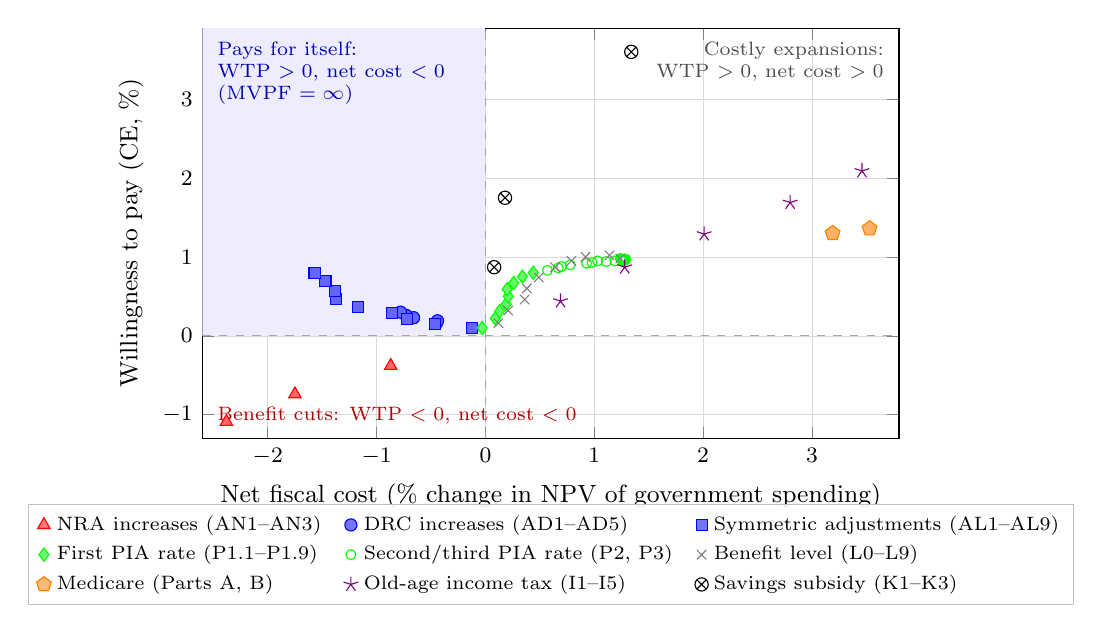
\begin{tikzpicture}
\begin{axis}[width=0.86\textwidth,height=0.56\textwidth,
  xmin=-2.6,xmax=3.8,ymin=-1.3,ymax=3.9,
  xlabel={Net fiscal cost (\% change in NPV of government spending)},
  ylabel={Willingness to pay (CE, \%)},
  grid=both,grid style={line width=.1pt, draw=gray!15},major grid style={line width=.2pt,draw=gray!30},
  tick label style={font=\footnotesize},label style={font=\small},
  legend style={font=\scriptsize,at={(0.99,0.02)},anchor=south east,draw=gray!50,fill=white,fill opacity=0.9,text opacity=1,cells={anchor=west}},
  legend cell align=left]
\fill[blue!7] (axis cs:-2.6,0) rectangle (axis cs:0,3.9);
\draw[gray!70,dashed] (axis cs:-2.6,0) -- (axis cs:3.8,0);
\draw[gray!70,dashed] (axis cs:0,-1.3) -- (axis cs:0,3.9);
\node[font=\scriptsize,align=left,anchor=north west,text=blue!70!black] at (axis cs:-2.55,3.85) {Pays for itself:\\ WTP $>0$, net cost $<0$\\ (MVPF $=\infty$)};
\node[font=\scriptsize,align=right,anchor=north east,text=black!70] at (axis cs:3.75,3.85) {Costly expansions:\\ WTP $>0$, net cost $>0$};
\node[font=\scriptsize,align=left,anchor=south west,text=red!70!black] at (axis cs:-2.55,-1.25) {Benefit cuts: WTP $<0$, net cost $<0$};
\addplot[only marks,mark=triangle*,mark size=2.6pt,color=red,mark options={solid,fill=red!60,draw=red}] coordinates {(-0.87,-0.38) (-1.75,-0.74) (-2.38,-1.09)};
\addlegendentry{NRA increases (AN1--AN3)}
\addplot[only marks,mark=*,mark size=2.2pt,color=blue,mark options={solid,fill=blue!60,draw=blue}] coordinates {(-0.45,0.16) (-0.44,0.19) (-0.66,0.23) (-0.73,0.26) (-0.78,0.3)};
\addlegendentry{DRC increases (AD1--AD5)}
\addplot[only marks,mark=square*,mark size=2.0pt,color=blue,mark options={solid,fill=blue!60,draw=blue}] coordinates {(-0.12,0.1) (-0.46,0.15) (-0.72,0.21) (-0.86,0.29) (-1.17,0.37) (-1.37,0.47) (-1.38,0.57) (-1.47,0.69) (-1.57,0.8)};
\addlegendentry{Symmetric adjustments (AL1--AL9)}
\addplot[only marks,mark=diamond*,mark size=2.4pt,color=green,mark options={solid,fill=green!60,draw=green}] coordinates {(-0.03,0.1) (0.09,0.22) (0.13,0.31) (0.19,0.4) (0.21,0.5) (0.2,0.59) (0.26,0.67) (0.34,0.75) (0.44,0.8)};
\addlegendentry{First PIA rate (P1.1--P1.9)}
\addplot[only marks,mark=o,mark size=1.8pt,color=green,mark options={solid,fill=green!60,draw=green}] coordinates {(0.57,0.83) (0.67,0.86) (0.7,0.88) (0.78,0.9) (0.93,0.92) (0.98,0.93) (1.03,0.95) (1.11,0.94) (1.19,0.95) (1.27,0.95) (1.26,0.95) (1.27,0.96) (1.28,0.96) (1.26,0.96) (1.27,0.96) (1.29,0.97) (1.27,0.97) (1.27,0.97) (1.25,0.97) (1.24,0.98)};
\addlegendentry{Second/third PIA rate (P2, P3)}
\addplot[only marks,mark=x,mark size=2.4pt,color=gray,mark options={solid,fill=gray!60,draw=gray}] coordinates {(0.12,0.16) (0.21,0.32) (0.36,0.46) (0.38,0.6) (0.49,0.74) (0.64,0.87) (0.79,0.95) (0.92,1) (1.14,1.02) (1.24,0.98)};
\addlegendentry{Benefit level (L0--L9)}
\addplot[only marks,mark=pentagon*,mark size=2.8pt,color=orange,mark options={solid,fill=orange!60,draw=orange}] coordinates {(3.53,1.36) (3.19,1.3)};
\addlegendentry{Medicare (Parts A, B)}
\addplot[only marks,mark=star,mark size=2.8pt,color=violet,mark options={solid,fill=violet!60,draw=violet}] coordinates {(0.69,0.44) (1.28,0.87) (2.01,1.29) (2.8,1.69) (3.46,2.09)};
\addlegendentry{Old-age income tax (I1--I5)}
\addplot[only marks,mark=otimes,mark size=2.4pt,color=black,mark options={solid,fill=black!60,draw=black}] coordinates {(0.08,0.87) (0.18,1.75) (1.34,3.6)};
\addlegendentry{Savings subsidy (K1--K3)}
\end{axis}
\end{tikzpicture}

\tabnotes{\textit{Notes:} Each marker is one reform of Tables~\ref{tab:claiming}, \ref{tab:generosity}, \ref{tab:generosity_app}, and~\ref{tab:other}. Horizontal axis: net fiscal cost, the percentage change in the present value of per capita government spending discounted to age 62 (Net). Vertical axis: willingness to pay, the ex ante consumption-equivalent welfare change at age 30, in percent (WTP). Shaded region: WTP $>0$ and net cost $<0$, where the MVPF is infinite. Lower-left quadrant: reforms that lower welfare and save money, for which the MVPF is the welfare cost per dollar saved. Upper-right quadrant: reforms that raise welfare at a positive net cost. For the reforms that start at age 62, the MVPF equals the slope of the ray from the origin times a common factor (Section~\ref{sec:fw_mvpf}). The savings subsidies use a different consumption base for their MVPFs, and their net costs treat capital income as taxed every period (\autoref{tab:other}). All entries come from simulations of the estimated model with prices held fixed.}
\end{figure}

The map has three regions. The shaded upper-left region contains the reforms that pay for themselves: all fourteen reforms that reward delay and the smallest expansion of the bottom bracket. Their savings are not small: the steepest symmetric reforms lie to the left of AN1. The lower-left quadrant contains the NRA increases, which lie on a flat ray: they save much per unit of welfare lost, but they lose welfare. The upper-right quadrant contains the costly expansions. Within it, the first-rate reforms lie above the level reforms at the same net cost; the reforms of the upper rates extend to the right at a nearly constant WTP, adding cost without adding welfare; the income-tax cuts lie along a ray of nearly constant slope, as their nearly constant MVPFs imply; and the Medicare expansions lie far to the right, on the flattest rays among the expansions.

Because the reforms that start at 62 share a common consumption base, their MVPFs can be ranked directly. Reforms that reward delay come first, with infinite MVPFs. Expansions of the bottom bracket follow, with MVPFs between 0.69 and 1.14 and an infinite MVPF for the smallest. Level reforms and increases in the upper rates follow at 0.29 to 0.61, then cuts in old-age income taxes at 0.23 to 0.26. A reduction of the NRA, the reverse of AN1--AN3, at 0.16 to 0.18, and the Medicare expansions, at 0.146 to 0.155, come last. The savings subsidies appear on the same axes, but their net costs rest on the upper-bound treatment of capital-income taxes, and Section~\ref{sec:discussion} places their MVPFs on the common base.

The ranking reflects two properties of a reform: whom it pays at unchanged behavior, and what it pays for at the margin. A credit for delay pays at the margin for delays that lower the program's outlays and pays nothing to those who cannot delay. The bottom bracket pays retirees whose lifetime earnings were depressed by low ability or poor health. A lower NRA pays every claimant, and an old-age tax cut pays in proportion to old-age income. A Medicare expansion pays for medical expenditures concentrated at the oldest ages, which drive its large cost.
